\documentclass{beamer}
\usetheme[alternativetitlepage=true]{Torino}

\author{Will Fuqua}
\title{\LaTeX{} Part II}
\institute{Michigan!/usr/group}
\date{December 2013}

\begin{document}

\begin{frame}[t,plain]
    \titlepage
\end{frame}

\begin{frame}[t]{What we'll cover about \LaTeX}
    \begin{itemize}
        \item How to write it
            \begin{itemize}
                \item Vim
                \item TexMaker
                \item Lyx
            \end{itemize}
            \pause
        \item What to write with it
            \begin{itemize}
                \item Articles
                \item Presentations 
                    (this presentation! \href{http://bit.ly/muglatex}{bit.ly/muglatex})
                \item R\'{e}sum\'{e}s
            \end{itemize}
            \pause
        \item Related topics
            \begin{itemize}
                \item ConTeXt
                \item Pandoc
            \end{itemize}
    \end{itemize}
\end{frame}

\begin{frame}{How to write it \textendash{} Vim}
    \begin{center}
        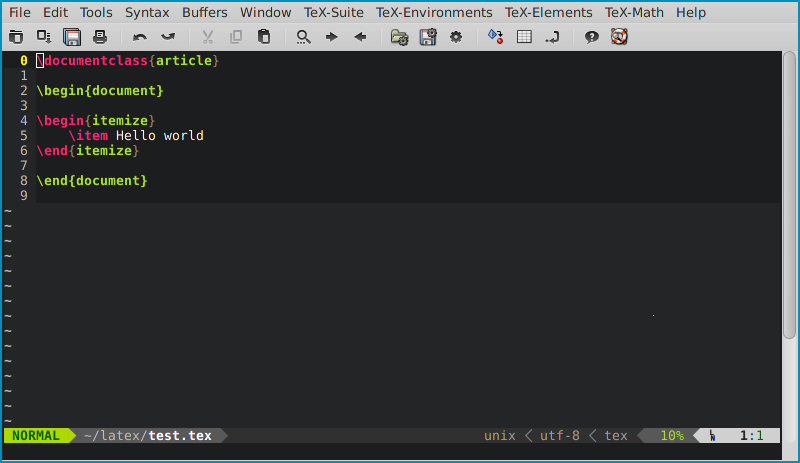
\includegraphics[width=0.8\textwidth]{img/vim}
    \end{center}
\end{frame}

\begin{frame}{How to write it \textendash{} TexMaker}
    \begin{center}
        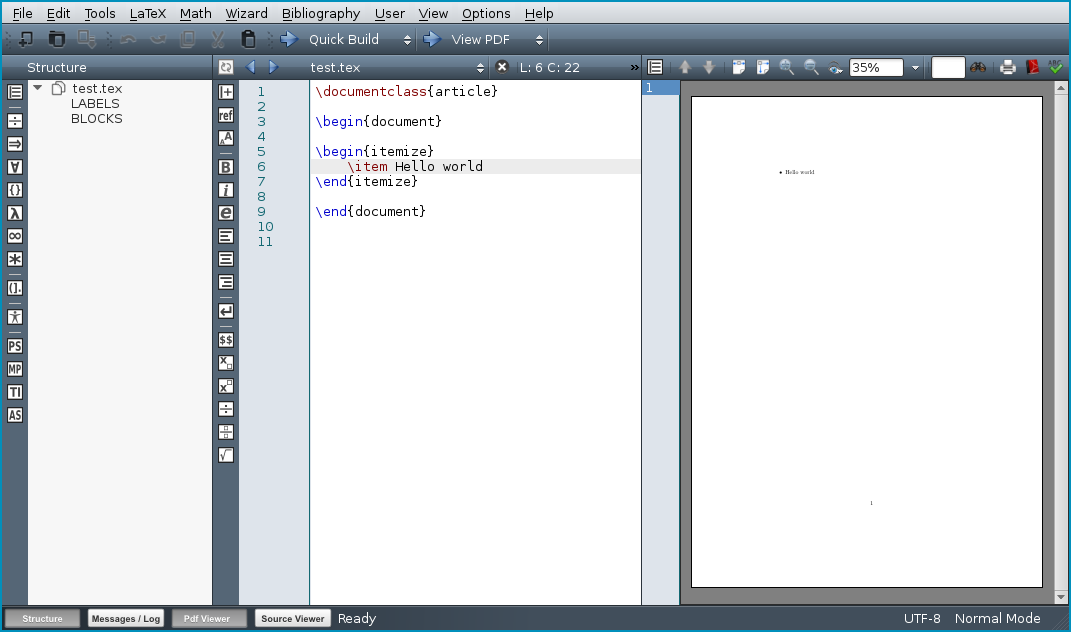
\includegraphics[width=0.8\textwidth]{img/texmaker}
    \end{center}
\end{frame}

\begin{frame}{How to write it \textendash{} Lyx}
    \begin{center}
        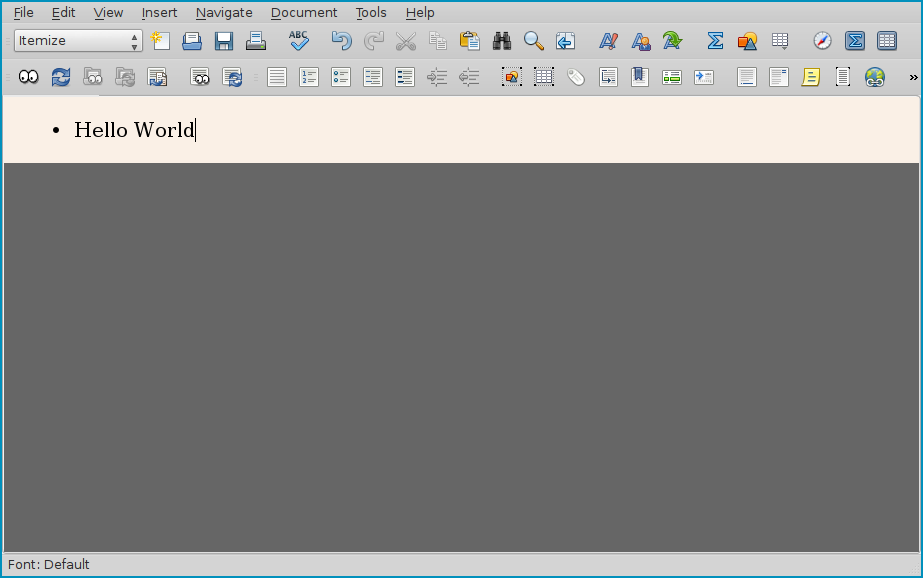
\includegraphics[width=0.8\textwidth]{img/lyx}
    \end{center}
\end{frame}

\begin{frame}{What to write with it \textendash{} Articles}
\end{frame}

\begin{frame}{What to write with it \textendash{} Presentations}
\end{frame}

\begin{frame}{What to write with it \textendash{} R\'{e}sum\'{e}s}
\end{frame}

\begin{frame}{Related topics \textendash{} ConTeXt}
\end{frame}

\begin{frame}{Related topics \textendash{} Pandoc}
\end{frame}
\end{document}

